%%%%%%%%%%%%%%%%%%%%%%%%%%%%%%%%%%%%%%%%%%%%%%%%%%%%%%%%%%%%%
%% HEADER
%%%%%%%%%%%%%%%%%%%%%%%%%%%%%%%%%%%%%%%%%%%%%%%%%%%%%%%%%%%%%
\documentclass[twoside]{report}

\usepackage{preamble}

\title{
GROOVE Documentation: \\
A Developer's Manual
}

\author{
Iovka Boneva, Harmen Kastenberg, Tom Staijen, and Arend Rensink \\
University of Twente\\
Department of Computer Science\\
\{bonevai,h.kastenberg,staijen,rensink\}@cs.utwente.nl
}

\date{\today}

% inlude headers
\pagestyle{headings}

% use roman page number for preface stuff
%\pagenumbering{roman}


\newtheorem{definition}{Definition}


%%%%%%%%%%%%%%%%%%%%%%%%%%%%%%%%%%%%%%%%%%%%%%%%%%%%%%%%%%%%%
%% DOCUMENT
%%%%%%%%%%%%%%%%%%%%%%%%%%%%%%%%%%%%%%%%%%%%%%%%%%%%%%%%%%%%%
\begin{document}

\maketitle

% we use the \cleardoublepage command whenever we start a new chapter in order
% to be sure that this chapter begins at the next available odd-numbered page
\cleardoublepage
\chapter*{Preface}

We are happy to present to you a document describing the fundamentals of the GROOVE Tool Set. In the coming pages we will provide the reader from a (hopefully) clear overview of the architecture of the tools within the GROOVE Tool Set.

Next to providing an overview of the structure of the tool, it is also meant as a starting point for those people just joining the GROOVE development team. We describe some basic principles that form the ground floor when writing new code for the tool, including some conventions which each developer should apply strictly.

For more information and downloads, we refer to the \GROOVE website: \url{http://groove.sourceforge.net/}

\vspace{0.2in}
\noindent
\hfill The GROOVE development team

\noindent
\hfill Enschede, The Netherlands

\tableofcontents

\cleardoublepage
% use arabic page numbering
%\pagenumbering{arabic}
% and start at 1
%\setcounter{page}{1}

\clearpage
\section{Introduction}

\GROOVE is a project centered around the use of simple graphs for modelling
any kind of dynamic system for which an abstract visual representation makes sense. The dynamics are specified through graph transformation rules. The core functionality of the tool is to explore all possible rule aplications, in a rich variety of ways, and to perform automatic verification (model checking).

This manual constsis of some download and installation instructions and a
manual for using the tools included in the \GROOVE tool set. The latter also
explains the format used for graphs and graph transformations. Together
with some examples, this should allow you to get started with \GROOVE.

\subsection{Toolkit Components}
\seclabel{toolkit}

The \GROOVE tool set includes the following tools:
\begin{description}\noitemsep
\item[Simulator:] a GUI-based tool that lets you construct, simulate and
  model check rule systems visually;
\item[Generator:] a command line tool that lets you simulate and model check
  rule systems without the performance penalty of the GUI;
\item[ModelChecker:] a command line tool for CTL model checking;
\item[PrologChecker:] a command line tool for executing Prolog queries on an explored grammar;
\item[Imager:] a command line or GUI tool that supports conversions from
  \GROOVE graphs and rules to other visual formats.
\item[Viewer:] a stand-alone (GUI) viewer for \GROOVE graphs and rules.
\end{description}

\subsection{Download}

The \GROOVE tool is distributed under the Apache License, Version 2.0. A copy
of this license is available on
\url{http://www.apache.org/licenses/LICENSE-2.0}.  The latest \GROOVE build
can be downloaded from the \GROOVE sourceforge page:

\begin{center}
\url{http://sourceforge.net/projects/groove}
\end{center}
%
There are some different packages available on the sourceforge site:
%
\begin{itemize}[noitemsep]
\item \textsf{groove}, the tool itself.
\item \textsf{groove-samples}, providing some sample grammars.
\item \textsf{groove-doc}, consisting of some publications about \GROOVE and
  the theory behind it.
\end{itemize}
%
\GROOVE depends on a number of other libraries, namely:

\DTLsetseparator{;}
\DTLloadrawdb[noheader,keys={name,description,url,version}]{libraries}{libraries.csv}

\begin{itemize}[noitemsep]
\DTLforeach{libraries}{%
  \libname=name,%
  \libdescr=description,%
  \liburl=url,%
  \libversion=version%
}{
\item \textsc{\libname}, for \libdescr. \\
  See \url{\liburl}%
  \ifthenelse{\equal{\libversion}{}}{}{ (Version included: \libversion)}%
  .
}
\end{itemize}

\subsection{Installation}

Since the entire \GROOVE tool is written in Java, getting it running is
extremely easy.

\medskip\noindent
To use the \GROOVE tool set, download the bin+lib package from the download
site explained above and unzip it to any location on your computer. Let's refer
to this location as the \GROOVE directory.

The \texttt{bin} subdirectory of the \GROOVE directory contains \texttt{jar}
files for each of the toolkit programs (see \secref{toolkit}), so
\texttt{Simulator.jar}, \texttt{Generator.jar} etc. You can use these in either of
the following ways:
\begin{itemize}
\item In an explorer window opened on the \texttt{bin} directory, double-click
  the icon of the \texttt{jar} file;
\item On the command line, run
%
\begin{verbatim}
java -jar GROOVE_PATH\bin\Program.jar [parameters]
\end{verbatim}
%
  where \texttt{GROOVE\_PATH} is the groove directory and \texttt{Program} is
  the toolkit program in question.
\end{itemize}


\cleardoublepage
\chapter{Background}
\chlabel{Background}


\section{The GROOVE project}

\GROOVE is an acronym of {\bf GR}aphs for {\bf O}bject {\bf O}riented {\bf VE}rification. In this project we work towards a method in which graphs are used for describing the structure of states of object-oriented programs. Such states mainly consist of objects that have been created during execution and their inter-relationships.

If each of the state of such a program is modelled by a single graph, the quesion is still how to relate (or order) all these graphs in a meaningful way. The obvious relation to chose is their temporal appearance. In other words, graphs representing subsequent states of a program should be related.

These relations between states are specified as applications of {\em graph transformation rules}. Intuitively, a graph transformation rule specifies how to make (local) changes to a certain graph. More formally, a graph transformation rule consists of a left hand side graph (\lhs) and a right hand side graph (\rhs) together with a graph morphism mapping elements of \lhs to elements of \rhs and a set of {\nac}s, being supergraphs of \lhs. It is not our intention to give an introduction to this field in this document, but rather refer to \cite{Heckel2006} which contains sufficient pointers for further reading.


\section{The GROOVE Approach}

Within the \GROOVE Tool Set the theory of graph transformation is applied on what are often called {\em simple graphs}. Simple graphs, as graphs in general, consists of a set of {\em nodes} and a set of {\em edges}. Edges, however, do not have an identity, but are identified by their {\em source node}, {\em target node}, and {\em label} instead. Therefore, edges with the same source node, target node, and label necessarily need to be equal, or stated differently, {\em parallel edges} are not allowed.

In \cite{GG-Handbook-I} the two main graph transformation approaches, namely the Single Pushout (\spo) and the Double Pushout (\dpo) approach, are explained and compared in detail. In \GROOVE we apply the \spo approach, mainly because the \dpo approach is not defined on simple graphs with partial graph morphisms. Shortly, the \spo approach unconditionally applies the graph transformation rules. If then, rule applications result in ill-formed graphs, i.e. graphs containing {\em dangling edges} for which either their source node or target node is not defined, those graphs are made well-formed again by removing the ill-formed part, i.e. by removing those dangling edges.

\section{Visualizing Transformation Rules}

Traditional graph transformation approaches specify a transformation rule by showing each component, i.e. its \lhs, \rhs, and all {\nac}s, separately. \fref{traditional-rule} is an example of such a traditional way of specifying a transformation rule. Graph morphisms are typically defined by means of the placing of the graph elements (i.e. nodes and edges).

\begin{figure}[htp]
  \centering
  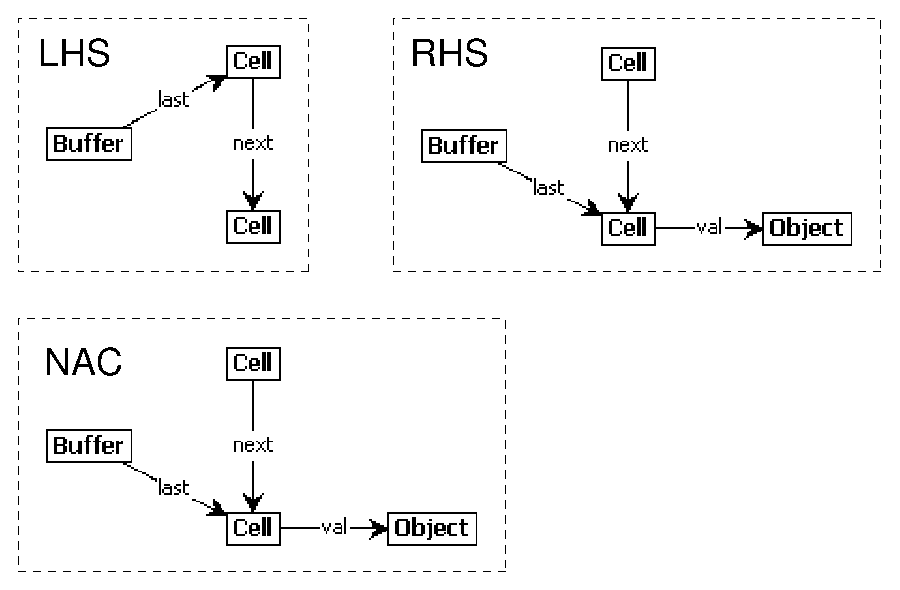
\includegraphics[scale=.75]{\figdir/traditional-rule}
  \caption{Traditional representation of a transformation rule.}
  \flabel{traditional-rule}
\end{figure}

In the GROOVE Tool Set we use a single graph representation of transformation rules. In this we depict the different roles of the graph elements by using different shapes and colours. We distinguish between four roles:

\begin{itemize}
  \item{{\em reader}: these are the nodes and edges that are only read by the rule, i.e. they are both in \lhs and \rhs. Reader nodes and edges are depicted as solid, black rectangles and arrows;}
  \item{{\em erasor}: these are the nodes and edges that are removed by the rule, i.e. they are only in \lhs. Erasor nodes and edges are represented by blue, dashed rectangles and arrows;}
  \item{{\em creator}: these are the nodes and edges that are created by the rule, i.e. they are only in \rhs. Creator nodes and edges are represented by solid, fat, green rectangles and arrows;}
  \item{{\em embargoe}: these are the nodes and edges that are forbidden for the rule to be applicable, i.e. they must not be present in the graph on which we want the rule to be applicable. Embargoe nodes and edges are represented by solid, fat, red rectangles and arrows.}
\end{itemize}

In \fref{groove-rule}, the single graph representation of the rule from \fref{traditional-rule} is shown.

\begin{figure}[htp]
  \centering
  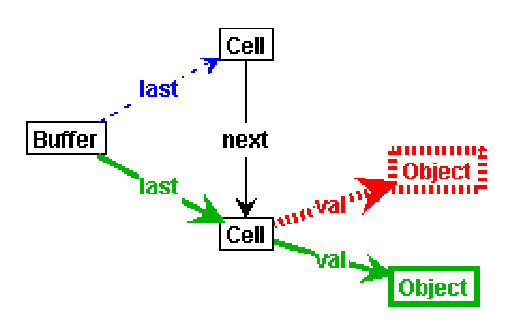
\includegraphics[scale=0.75]{\figdir/groove-rule}
  \caption{The GROOVE's single graph representation of \fref{traditional-rule}.}
  \flabel{groove-rule}
\end{figure}



\cleardoublepage
\chapter{The GROOVE Tool Set}
\chlabel{The GROOVE Tool Set}

\section{Tool Chain}

The GROOVE Tool Set basically consists of the following components:

\begin{itemize}
  \item{the simulator,}
  \item{the editor,}
  \item{the generator,}
  \item{the imager, and}
  \item{the model checker.}
\end{itemize}

\fref{tool-chain} gives an overview of how most of these tools work together, what they expect as input, and what they provide as output. The squares represent those parts of the tools that have been implemented (white background) and are planned in the future (gray background). The elipses represent the inputs and outputs for the different components.

In the following paragraphs we will shortly discuss all the implemented components, i.e. what they require as input and what they provide as output.

\begin{figure}
  \centering
  \includegraphics[scale=0.7]{\figdir/chain}
  \caption{Chain overview of the \GROOVE Tool Set.}
  \flabel{tool-chain}
\end{figure}

\section{The GROOVE Simulator}

The \GROOVE Simulator is a graphical interface enabling the user to control the \GROOVE transformation engine. It provides a direct graphical view on the state graphs, the transformation rules, and the part of the state space explored so far. Furthermore, from the Simulator the user is able to perform various actions on transformation rules, such as editing, disabling, removing, and creating new ones.

\paragraph{Input.} When starting the Simulator, it can be provided from a path to some directory containing a graph production system. Such directories should have the \texttt{.gps} `extension', otherwise the Simulator will not be able to load it succesfully. These graph production systems typically contain a (possibly empty) set of transformation rules together with a start graph named \texttt{start.gst}. When starting the Simulator from the command-line, it is possible to provide it from a different start graph, which may not be in the same directory as the transformation rules are in.

\paragraph{Output.} Apart from the visual feedback, the Simulator does not automatically provide physical output in the sense of log-files, for instance. At any point during the execution of the production system, it is possible to export the state graphs or individual rules or the transition system generated so far, to a GXL-file.


\section{The GROOVE Editor}

The GROOVE Editor provides means for specifying graphs and transformation rules. From the Editor one is able to create new or modify existing graphs and rules. It does not require any input. Its output consists of the graphs and transformation rules saved by the user.


\section{The GROOVE Generator}

The GROOVE Generator is a useful tool when users are only interested in the outcome of applying the rules of a production system to a specific graph as long as possible, without the need to look at the transformation process itself.

For example, when providing the Generator from a graph production system, it can be asked to save all the final states, i.e. the states in which no rule is applicable anymore.

\paragraph{Input.} The required input is the same as for the Simulator, i.e. a path to the directory containing a graph production system. The Generator can also be provided from a different start graph. Furthermore, the Generator has some options for directing the transformation process. These are, among others, the strategy to use for the transformation process and a file to write the results to.

\paragraph{Output.} When the Generator has finished, it should have written the required result to the specified location. Optionally, it creates a log-file containing some statistics about the transformation process.


\section{The GROOVE Imager}

With the GROOVE Imager one is able to create images from both graphs and transformation rules in various formats, such as JPG, PNG, and EPS.

\section{The GROOVE Model Checker}

Currently, the GROOVE Model Checker supports the verification of properties specified as CTL formulae over finite state graph production systems.

The Model Checker is a command-line tool which, given a graph production system generating a finite state space, first does the state space generation and subsequently asks the user for properties to be verified over this state space. The user is able to check multiple properties in sequence without the need to generate the state space over and over again.

\paragraph{Input.} The input for the Model Checker is equivalent to that of the Generator. After the transformation process, the user is asked to enter CTL formulae that have to be checked, or quit the program.

\paragraph{Output.} Currently, the Model Checker only provides output stating that a given temporal formula is satisfied by the system as specified by the graph production system or is not satisfied.

\cleardoublepage
\chapter{Tool Architecture}
\chlabel{Tool Architecture}

In this chapter we will discuss the internal structure of the \GROOVE Tool. We will explain the different Java packages all classes and interfaces are spread over.

\section{Packages}

\tblref{packages} enumerates the different packages (in alphabetical order) and gives a short description for each of them.

\begin{table}[htp]
  \centering
  \begin{tabular}{|c|p{3.5in}|}
  \hline
    {\bf Name} & {\bf Description} \\
    \hline
    \hline
    {\tt groove.algebra} & package providing the algebraic structure for attributed graphs \\
    \hline
    {\tt groove.calc} & package providing classes using graph transformations as a calculation tool \\
    \hline
    {\tt groove.graph} & package containing the basic interfaces and classes implementing graphs using different internal structures \\
    {\tt groove.graph.algebra} & package providing the necessary graph elements for attributed graphs \\
    {\tt groove.graph.aspects} & \\
    {\tt groove.graph.iso} & package providing functionality for determining isomorphism relations between graphs based on {\em graph certificates} \\
    \hline
    {\tt groove.gui} & package containing the classes implementing the graphical user interface of the \GROOVE Tool Set \\
    {\tt groove.gui.jgraph} & package containing classes that serve as an intermediate level between the \GROOVE transformation engine and the JGraph third party library used for visialization \\
    {\tt groove.gui.layout} & package providing classes to manage different graph layout algorithms \\
    \hline
    {\tt groove.gxl} & \\
    {\tt groove.gxl.types} & \\
    \hline
    {\tt groove.io} & package containing I/O classes, i.e. xml marshallers and unmarshallers \\
    \hline
    {\tt groove.lts} & \\
    {\tt groove.lts.explore} & \\
    \hline
    {\tt groove.rel} & package containing interfaces and classes featuring the use of regular expressions in transformation rules \\
    \hline
    {\tt groove.samples} & \\
    \hline
    {\tt groove.test} & package containing JUnit classes for testing the GROOVE Tool Set \\
    {\tt groove.test.graph} & subpackage containing specialized test-classes for different graph implementations \\
    \hline
    {\tt groove.trans} & package containing interfaces and classes that form the actual graph transformation engine \\
    {\tt groove.trans.view} & package providing functionality for displaying transformation rules in the typical \GROOVE single-graph representation \\
    \hline
    {\tt groove.util} & package providing small utilities used internally throughout the \GROOVE Tool Set \\
    {\tt groove.verify} & package containing interfaces and classes providing the model checking functionality of the \GROOVE Tool Set \\
    \hline
  \end{tabular}
  \caption{Overview of Java-packages within the \GROOVE Tool Set.}
  \tbllabel{packages}
\end{table}

\section{Class Hierarchies}

\subsection{Graphs}

The notion of graphs can be used at different levels. Especially in \GROOVE, we distinghuis between ordinary graphs just consisting of nodes and labeled and directed edges. On the other hand, we also use graphs to model {\em transition systems} in which the nodes are graphs themselves and edges represent rule applications. In order to make this possible, the \Graph-interface has different sub-interfaces as shown in \fref{graph-hierarchy}.

\begin{figure}
  \centering
  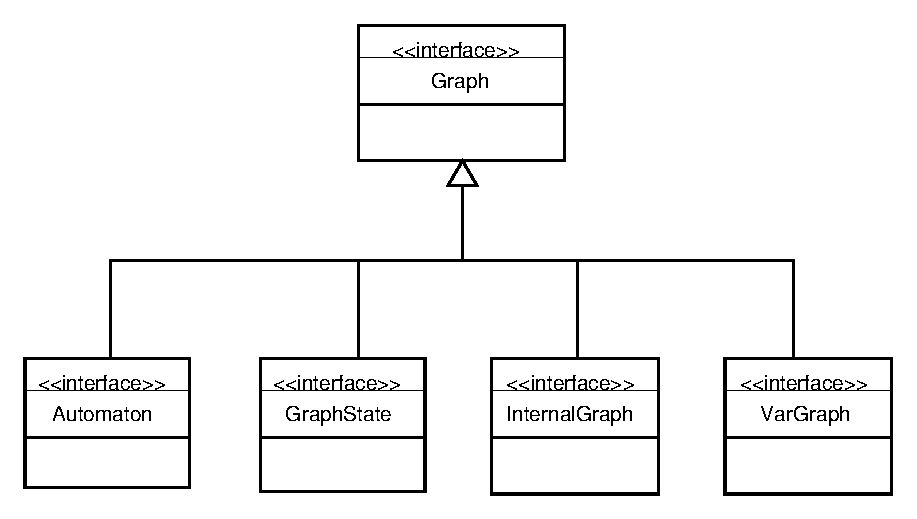
\includegraphics[scale=0.7]{\figdir/graph-hierarchy}
  \caption{The \Graph interface with different sub-interfaces.}
  \flabel{graph-hierarchy}
\end{figure}

Within the GROOVE Tool Set different implementations of graph structures are available. They mainly differ in the way they access their components. \fref{graph-hierarchy} gives an overview of the most frequently used graph implementations. For each of these we will explain the idea behind those specific implementations.

\subsection{Applied Patterns}

\subsubsection{Model View Controller}

%\cleardoublepage
%\section{License}
\alabel{license}

The GROOVE tool is distributed under the terms of the GNU General Public
License which terms and conditions are given hereafter.


\subsection*{The GNU General Public License}
\begin{center}
{\parindent 0in

Version 2, June 1991

Copyright \copyright\ 1989, 1991 Free Software Foundation, Inc.

\bigskip

51 Franklin St, Fifth Floor, Boston, MA  02110-1301, USA

\bigskip

Everyone is permitted to copy and distribute verbatim copies
of this license document, but changing it is not allowed.
}
\end{center}

\renewcommand{\abstractname}{Preamble}
\begin{abstract}
The licenses for most software are designed to take away your freedom to
share and change it.  By contrast, the GNU General Public License is
intended to guarantee your freedom to share and change free software---to
make sure the software is free for all its users.  This General Public
License applies to most of the Free Software Foundation's software and to
any other program whose authors commit to using it.  (Some other Free
Software Foundation software is covered by the GNU Library General Public
License instead.)  You can apply it to your programs, too.

When we speak of free software, we are referring to freedom, not price.
Our General Public Licenses are designed to make sure that you have the
freedom to distribute copies of free software (and charge for this service
if you wish), that you receive source code or can get it if you want it,
that you can change the software or use pieces of it in new free programs;
and that you know you can do these things.

To protect your rights, we need to make restrictions that forbid anyone to
deny you these rights or to ask you to surrender the rights.  These
restrictions translate to certain responsibilities for you if you
distribute copies of the software, or if you modify it.

For example, if you distribute copies of such a program, whether gratis or
for a fee, you must give the recipients all the rights that you have.  You
must make sure that they, too, receive or can get the source code.  And
you must show them these terms so they know their rights.

We protect your rights with two steps: (1) copyright the software, and (2)
offer you this license which gives you legal permission to copy,
distribute and/or modify the software.

Also, for each author's protection and ours, we want to make certain that
everyone understands that there is no warranty for this free software.  If
the software is modified by someone else and passed on, we want its
recipients to know that what they have is not the original, so that any
problems introduced by others will not reflect on the original authors'
reputations.

Finally, any free program is threatened constantly by software patents.
We wish to avoid the danger that redistributors of a free program will
individually obtain patent licenses, in effect making the program
proprietary.  To prevent this, we have made it clear that any patent must
be licensed for everyone's free use or not licensed at all.

The precise terms and conditions for copying, distribution and
modification follow.
\end{abstract}

\begin{center}
{\Large \sc GNU General Public License
\\\vspace{3mm}Terms and Conditions For Copying, Distribution and Modification}
\end{center}


\begin{enumerate}

\addtocounter{enumi}{-1}

\item 

This License applies to any program or other work which contains a notice
placed by the copyright holder saying it may be distributed under the
terms of this General Public License.  The ``Program'', below, refers to
any such program or work, and a ``work based on the Program'' means either
the Program or any derivative work under copyright law: that is to say, a
work containing the Program or a portion of it, either verbatim or with
modifications and/or translated into another language.  (Hereinafter,
translation is included without limitation in the term ``modification''.)
Each licensee is addressed as ``you''.

Activities other than copying, distribution and modification are not
covered by this License; they are outside its scope.  The act of
running the Program is not restricted, and the output from the Program
is covered only if its contents constitute a work based on the
Program (independent of having been made by running the Program).
Whether that is true depends on what the Program does.

\item You may copy and distribute verbatim copies of the Program's source
  code as you receive it, in any medium, provided that you conspicuously
  and appropriately publish on each copy an appropriate copyright notice
  and disclaimer of warranty; keep intact all the notices that refer to
  this License and to the absence of any warranty; and give any other
  recipients of the Program a copy of this License along with the Program.

You may charge a fee for the physical act of transferring a copy, and you
may at your option offer warranty protection in exchange for a fee.

\item

You may modify your copy or copies of the Program or any portion
of it, thus forming a work based on the Program, and copy and
distribute such modifications or work under the terms of Section 1
above, provided that you also meet all of these conditions:

\begin{enumerate}

\item 

You must cause the modified files to carry prominent notices stating that
you changed the files and the date of any change.

\item

You must cause any work that you distribute or publish, that in
whole or in part contains or is derived from the Program or any
part thereof, to be licensed as a whole at no charge to all third
parties under the terms of this License.

\item
If the modified program normally reads commands interactively
when run, you must cause it, when started running for such
interactive use in the most ordinary way, to print or display an
announcement including an appropriate copyright notice and a
notice that there is no warranty (or else, saying that you provide
a warranty) and that users may redistribute the program under
these conditions, and telling the user how to view a copy of this
License.  (Exception: if the Program itself is interactive but
does not normally print such an announcement, your work based on
the Program is not required to print an announcement.)

\end{enumerate}


These requirements apply to the modified work as a whole.  If
identifiable sections of that work are not derived from the Program,
and can be reasonably considered independent and separate works in
themselves, then this License, and its terms, do not apply to those
sections when you distribute them as separate works.  But when you
distribute the same sections as part of a whole which is a work based
on the Program, the distribution of the whole must be on the terms of
this License, whose permissions for other licensees extend to the
entire whole, and thus to each and every part regardless of who wrote it.

Thus, it is not the intent of this section to claim rights or contest
your rights to work written entirely by you; rather, the intent is to
exercise the right to control the distribution of derivative or
collective works based on the Program.

In addition, mere aggregation of another work not based on the Program
with the Program (or with a work based on the Program) on a volume of
a storage or distribution medium does not bring the other work under
the scope of this License.

\item
You may copy and distribute the Program (or a work based on it,
under Section 2) in object code or executable form under the terms of
Sections 1 and 2 above provided that you also do one of the following:

\begin{enumerate}

\item

Accompany it with the complete corresponding machine-readable
source code, which must be distributed under the terms of Sections
1 and 2 above on a medium customarily used for software interchange; or,

\item

Accompany it with a written offer, valid for at least three
years, to give any third party, for a charge no more than your
cost of physically performing source distribution, a complete
machine-readable copy of the corresponding source code, to be
distributed under the terms of Sections 1 and 2 above on a medium
customarily used for software interchange; or,

\item

Accompany it with the information you received as to the offer
to distribute corresponding source code.  (This alternative is
allowed only for noncommercial distribution and only if you
received the program in object code or executable form with such
an offer, in accord with Subsection b above.)

\end{enumerate}


The source code for a work means the preferred form of the work for
making modifications to it.  For an executable work, complete source
code means all the source code for all modules it contains, plus any
associated interface definition files, plus the scripts used to
control compilation and installation of the executable.  However, as a
special exception, the source code distributed need not include
anything that is normally distributed (in either source or binary
form) with the major components (compiler, kernel, and so on) of the
operating system on which the executable runs, unless that component
itself accompanies the executable.

If distribution of executable or object code is made by offering
access to copy from a designated place, then offering equivalent
access to copy the source code from the same place counts as
distribution of the source code, even though third parties are not
compelled to copy the source along with the object code.

\item
You may not copy, modify, sublicense, or distribute the Program
except as expressly provided under this License.  Any attempt
otherwise to copy, modify, sublicense or distribute the Program is
void, and will automatically terminate your rights under this License.
However, parties who have received copies, or rights, from you under
this License will not have their licenses terminated so long as such
parties remain in full compliance.

\item
You are not required to accept this License, since you have not
signed it.  However, nothing else grants you permission to modify or
distribute the Program or its derivative works.  These actions are
prohibited by law if you do not accept this License.  Therefore, by
modifying or distributing the Program (or any work based on the
Program), you indicate your acceptance of this License to do so, and
all its terms and conditions for copying, distributing or modifying
the Program or works based on it.

\item
Each time you redistribute the Program (or any work based on the
Program), the recipient automatically receives a license from the
original licensor to copy, distribute or modify the Program subject to
these terms and conditions.  You may not impose any further
restrictions on the recipients' exercise of the rights granted herein.
You are not responsible for enforcing compliance by third parties to
this License.

\item
If, as a consequence of a court judgment or allegation of patent
infringement or for any other reason (not limited to patent issues),
conditions are imposed on you (whether by court order, agreement or
otherwise) that contradict the conditions of this License, they do not
excuse you from the conditions of this License.  If you cannot
distribute so as to satisfy simultaneously your obligations under this
License and any other pertinent obligations, then as a consequence you
may not distribute the Program at all.  For example, if a patent
license would not permit royalty-free redistribution of the Program by
all those who receive copies directly or indirectly through you, then
the only way you could satisfy both it and this License would be to
refrain entirely from distribution of the Program.

If any portion of this section is held invalid or unenforceable under
any particular circumstance, the balance of the section is intended to
apply and the section as a whole is intended to apply in other
circumstances.

It is not the purpose of this section to induce you to infringe any
patents or other property right claims or to contest validity of any
such claims; this section has the sole purpose of protecting the
integrity of the free software distribution system, which is
implemented by public license practices.  Many people have made
generous contributions to the wide range of software distributed
through that system in reliance on consistent application of that
system; it is up to the author/donor to decide if he or she is willing
to distribute software through any other system and a licensee cannot
impose that choice.

This section is intended to make thoroughly clear what is believed to
be a consequence of the rest of this License.

\item
If the distribution and/or use of the Program is restricted in
certain countries either by patents or by copyrighted interfaces, the
original copyright holder who places the Program under this License
may add an explicit geographical distribution limitation excluding
those countries, so that distribution is permitted only in or among
countries not thus excluded.  In such case, this License incorporates
the limitation as if written in the body of this License.

\item
The Free Software Foundation may publish revised and/or new versions
of the General Public License from time to time.  Such new versions will
be similar in spirit to the present version, but may differ in detail to
address new problems or concerns.

Each version is given a distinguishing version number.  If the Program
specifies a version number of this License which applies to it and ``any
later version'', you have the option of following the terms and conditions
either of that version or of any later version published by the Free
Software Foundation.  If the Program does not specify a version number of
this License, you may choose any version ever published by the Free Software
Foundation.

\item
If you wish to incorporate parts of the Program into other free
programs whose distribution conditions are different, write to the author
to ask for permission.  For software which is copyrighted by the Free
Software Foundation, write to the Free Software Foundation; we sometimes
make exceptions for this.  Our decision will be guided by the two goals
of preserving the free status of all derivatives of our free software and
of promoting the sharing and reuse of software generally.

\begin{center}
{\Large\sc
No Warranty
}
\end{center}

\item
{\sc Because the program is licensed free of charge, there is no warranty
for the program, to the extent permitted by applicable law.  Except when
otherwise stated in writing the copyright holders and/or other parties
provide the program ``as is'' without warranty of any kind, either expressed
or implied, including, but not limited to, the implied warranties of
merchantability and fitness for a particular purpose.  The entire risk as
to the quality and performance of the program is with you.  Should the
program prove defective, you assume the cost of all necessary servicing,
repair or correction.}

\item
{\sc In no event unless required by applicable law or agreed to in writing
will any copyright holder, or any other party who may modify and/or
redistribute the program as permitted above, be liable to you for damages,
including any general, special, incidental or consequential damages arising
out of the use or inability to use the program (including but not limited
to loss of data or data being rendered inaccurate or losses sustained by
you or third parties or a failure of the program to operate with any other
programs), even if such holder or other party has been advised of the
possibility of such damages.}

\end{enumerate}


\begin{center}
{\Large\sc End of Terms and Conditions}
\end{center}


\pagebreak[2]

\subsection*{Appendix: How to Apply These Terms to Your New Programs}

If you develop a new program, and you want it to be of the greatest
possible use to the public, the best way to achieve this is to make it
free software which everyone can redistribute and change under these
terms.

  To do so, attach the following notices to the program.  It is safest to
  attach them to the start of each source file to most effectively convey
  the exclusion of warranty; and each file should have at least the
  ``copyright'' line and a pointer to where the full notice is found.

\begin{verbatim}
<one line to give the program's name and a brief idea of what it does.> 
Copyright (C) <year>  <name of author> 

This program is free software; you can redistribute it and/or modify
it under the terms of the GNU General Public License as published by
the Free Software Foundation; either version 2 of the License, or
(at your option) any later version.

This program is distributed in the hope that it will be useful,
but WITHOUT ANY WARRANTY; without even the implied warranty of
MERCHANTABILITY or FITNESS FOR A PARTICULAR PURPOSE.  See the
GNU General Public License for more details.

You should have received a copy of the GNU General Public License
along with this program; if not, write to the Free Software
Foundation, Inc., 51 Franklin St, Fifth Floor, Boston, MA  02110-1301, USA.
\end{verbatim}

Also add information on how to contact you by electronic and paper mail.

If the program is interactive, make it output a short notice like this
when it starts in an interactive mode:

\begin{verbatim}
Gnomovision version 69, Copyright (C) <year>  <name of author> 
Gnomovision comes with ABSOLUTELY NO WARRANTY; for details type `show w'. 
This is free software, and you are welcome to redistribute it
under certain conditions; type `show c' for details.
\end{verbatim}


The hypothetical commands {\tt show w} and {\tt show c} should show the
appropriate parts of the General Public License.  Of course, the commands
you use may be called something other than {\tt show w} and {\tt show c};
they could even be mouse-clicks or menu items---whatever suits your
program.

You should also get your employer (if you work as a programmer) or your
school, if any, to sign a ``copyright disclaimer'' for the program, if
necessary.  Here is a sample; alter the names:

\begin{verbatim}
Yoyodyne, Inc., hereby disclaims all copyright interest in the program
`Gnomovision' (which makes passes at compilers) written by James Hacker.

<signature of Ty Coon>, 1 April 1989 
Ty Coon, President of Vice
\end{verbatim}


This General Public License does not permit incorporating your program
into proprietary programs.  If your program is a subroutine library, you
may consider it more useful to permit linking proprietary applications
with the library.  If this is what you want to do, use the GNU Library
General Public License instead of this License.


\cleardoublepage
\chapter{Guidelines}
\chlabel{Guidelines}


\section{Documentation}

One of the most important things in programming is good and consistent documentation. Javadoc provides a good starting point for this. We therefore require all classes, methods, and fields to be accompanied with appropriate descriptions of their intent, possibly with cross-references to other Java classes.

\section{Package Size and Dependencies}

The basic guideline for packages is to keep the number of classes within reasonable size. The exact maximum number of classes within a package is of course debatable, but this number should never exceed e.g. 100.

Concerning the dependency relations between packages we can be more clear. The basic guideline is to have only {\em one-directional} dependencies between packages.


\section{Coding Conventions}

For accessing class fields we apply the following guidelines. The general principle is that of {\em lazy initialization}. This means that whenever accessing a field \x through its \getX-method, we will first check whether \x has already been initialized or is still \nullPnt. If it is \nullPnt, we call the (protected) \computeX-method. The \computeX-method first calls the \createX-method after which it may still need to do some additional computations. The \createX-method only creates a new instance of the correct type.

Listing \ref{l:X-lazy.java} gives an overview of the things discussed above.

\codelisting{java}{X-lazy.java}{Lazy initialization.}

\subsection{Method Level}

\section{Peer Reviews}

Keeping code clear and understandable requires quite a lot of effort. In order to decentralize this process, developers can now and then schedule so called `code reviews'. Code reviews are performed on pieces of code written by other developers. When things are unclear this should be indicated by what we call {\em personal tags}.

\subsection{Personal Tags}

In order to be able to keep track of code being reviewed, individual tags have been introduced for each developer. That is, whenever you review a class or method and want to add some comments, you should include your personal tag (your first name in capital letters) followed by the actual comment. The idea is then that every now and then, developers should take a quick look at all the comments and see whether some comments require some discussion or simple actions to be taken. The use of personal tags is shown in Listing \ref{l:X.java}.

\codelisting{java}{X.java}{Personal tags.}


\cleardoublepage
\chapter{Data Structures and Algorithms}
\chlabel{Data Structures and Algorithms}

In this chapter we give a description to some of the most complex
algorithms and data structures in the \GROOVE implementation. This should
help the developer to have a relatively high-level view on \GROOVE. This
description is to be considered together with the {\em javadoc} that gives
a detailed explanations on the classes / methods, that we do not reproduce
here.

\section{Storage of Graphs}
\stlabel{storage of graphs}

The tool \GROOVE manipulates a labelled transition system that may contain
a very big number of graphs as states. Space is a critical resource for the
tool, and efficient storage of graphs is essential.

There are two essential mechanisms in \GROOVE that are related to efficient
graph storage, while trying to keep an optimal time performance:
\begin{itemize}
\item a {\em delta graph} is a representation of a graph expressed by the
  changes that one should operate on some {\em basis graph} in order to
  obtain it. {\em Changes} are added and removed elements (nodes or edges).
  Delta graphs are very useful as in a labelled transition system most of
  the new graphs are generated by graph transformation, thus share lots of
  common structure with other graphs. This is the format in which graphs
  are represented in run-time;
\item a {\em graph cache} is a representation of a graph as a set of nodes
  and a set of edges with additional information in order to make graph
  processing easier. If the JVM runs out of memory, the garbage collector
  is authorised to remove cache graphs. If some computations with a graph
  are involved, then the cache is recomputed again.
\end{itemize}

On \fref{graphs} we depict the class hierarchy relative to the
representation of graphs and delta graphs in \GROOVE. On \fref{elements} is
represented partially the class hierarchy relative to graph elements
(nodes, edges). Finally, \fref{caches} gives a portion of the class
hierarchy related to graph caches. For further details, we refer to the
{\em javadoc}.
\begin{figure}[ht]
  \centering
  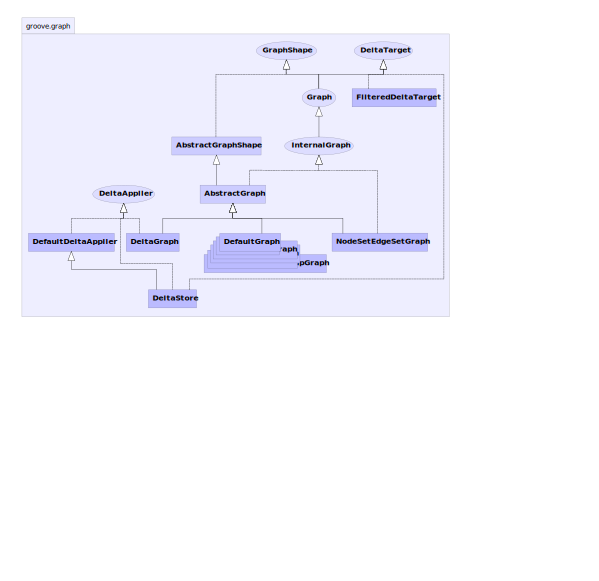
\includegraphics{fig/graphs}
  \caption{Graph related class hierarchy.}
  \flabel{graphs}
\end{figure}

\begin{figure}[ht]
  \centering
  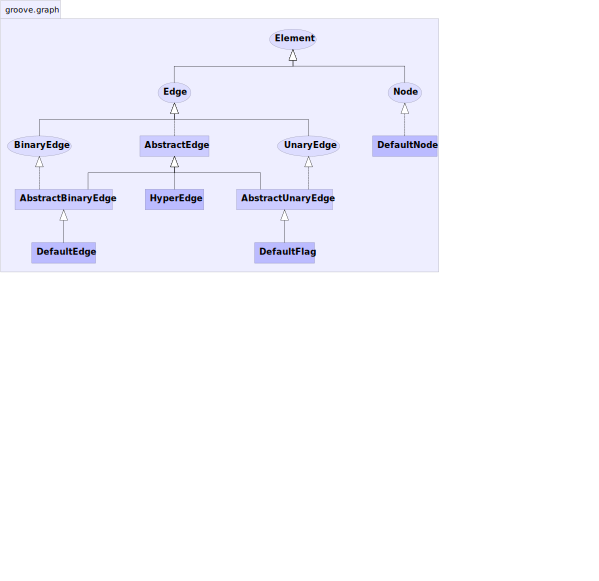
\includegraphics{fig/elements}
  \caption{Part of the class hierarchy relative to graph elements.}
  \flabel{elements}
\end{figure}

\begin{figure}[ht]
  \centering
  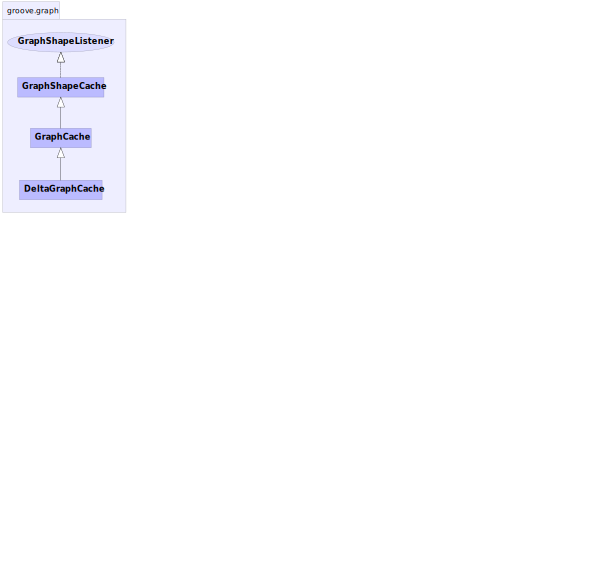
\includegraphics{fig/caches}
  \caption{Part of the class hierarchy relative to graph cache.}
  \flabel{caches}
\end{figure}

\paragraph{Delta Graph}
A {\em delta graph} is essentially a basis graph together with a set of
added elements and a set of removed elements (nodes or edges). For storage
optimisation, added and removed elements are stored into a single array,
called {\em delta array}. The basis graph can also be a delta graph.  Thus,
we can have a sequence of delta graphs, each of which is used as a basis of
the next one. Very long such sequences may result in a big loss of time
efficiency, as most of the manipulations on a graph require a node-set
edge-set based representation, which should be recomputed. Therefore, the
length of such sequences is limited to at most {\tt
  graph.DeltaGraphCache.FREEZE\_DEPTH}, currently set to $8$.
% TODO : what is a frozen delta graph ?
% TODO : make sure that it is indeed the limit

\paragraph{Graph Cache}
A graph cache is a representation of a graph that contains explicitly the
sets of nodes and edges of the graph, as well as adjacency map associating
with each node its adjacent edges, and edge label map, associating with
each label the edges wearing this label. This redundant representation
facilitates computations on a graph. 

An object of type {\tt graph.AbstractGraphShape} contains a reference to a
{\tt graph.GraphShapeCache} (in the form of a {\tt
  java.lang.ref.Reference<GraphShapeCache>} object), and it supports a {\tt
  clearCache()} operation that allows to notify the garbage collector that
the cache object can be collected in case there is a need of additional
memory.

\section{Labelled Transition System}

Remind that the \GROOVE Simulator and Generator allow to (partially)
construct the labelled transition system corresponding to some graph
grammar. Such a LTS is of the form $\mathcal S = (S, T, s_0, F)$. States in
$S$ are graphs and transitions in $T$ are of the form $(G, (P,m), H)$,
where the graphs $G,H$ are states of the labelled transition system and the
label $(P,m)$ consists of a graph production $P$ and a matching $m: L \to
G$ (with $P = (L, R)$).

The functionality of Groove related to computing and storing a Labelled
Transition System (LTS) is implemented into two packages.
\begin{itemize}
\item \texttt{lts} package for construction and storage of a labelled transition system,
\item \texttt{trans} package for computing transformations.
\end{itemize}
In what follows we describe these implementations. We start with a general
description, and then give details on the implementations. We omit the {\tt
  groove} prefix in class names (i.e. we write {\tt lts.GTS} instead of
{\tt groove.lts.GTS}).

\subsection{Interface for a Labelled Transition System}
A LTS is a graph-like structure. The interface {\tt graph.GraphShape}
defines basic graph functionality, such as adding, removing and retrieving
nodes and edges and sets of nodes and edges, etc. The interface {\tt
  lts.LTS} (\fref{lts-interface}) extends the interface {\tt
  graph.GraphShape} with the notion of start and final states and with the
method

\smallskip\noindent%
{\tt boolean isOpen(State state);}

\noindent
A state of a LTS is considered {\em open} if not all outgoing transitions have
not been explored.

\begin{figure}[ht]
  \centering
  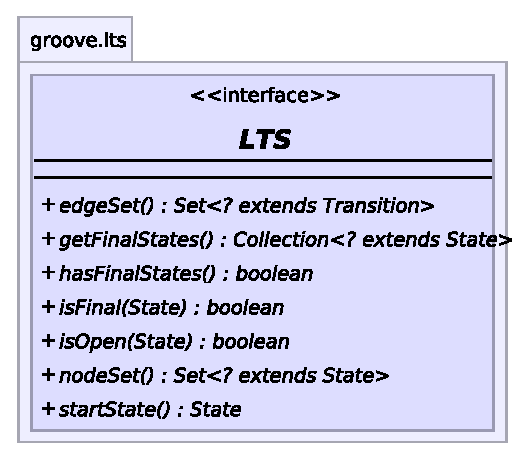
\includegraphics[scale=0.8]{fig/LTS}
  \caption{The interface {\tt lts.LTS}.}
  \flabel{lts-interface}
\end{figure}


\paragraph{States and Transitions of a Labelled Transition System}

The {\tt lts} package provides the hierarchy of states and
transitions of an LTS depicted on \fref{states and transitions}.

\begin{figure}[ht]
  \centering
  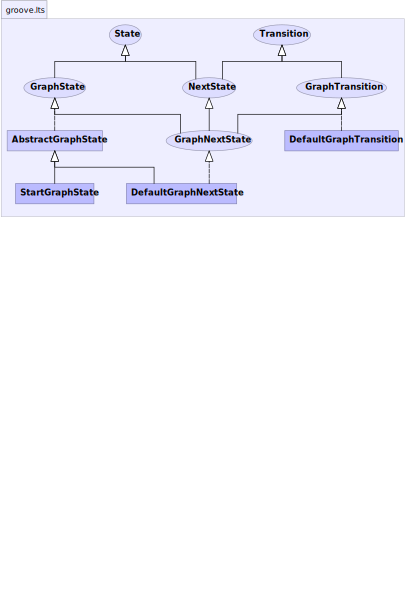
\includegraphics{fig/states-and-transitions}
  \caption{States and transitions class hierarchy for a LTS.}
  \flabel{states and transitions}
\end{figure}

The interface {\tt lts.NextState} combines a state and a transition. It is
intended to represent a state together with one of its incoming
transitions. The interface {\tt lts.GraphState}, {\tt lts.GraphTransition}
and {\tt lts.GraphNextState} specialise a state, a transition and a ``next
state'' for labelled transition systems which states are graphs and which
transitions represent direct derivations. The classes {\tt
  lts.DefaultGraphTransition}, {\tt lts.DefaultGraphNextState} and {\tt
  lts.StartGraphState} are the implementations of these interfaces. On
\fref{graphstate} we present in more detail the functionality provided by
the interface {\tt lts.GraphState}. As one can see from this figure, a {\tt
  lts.GraphState} knows its outgoing transitions. The {\tt setClosed()}
method closes the state, forbidding to add more outgoing transitions to it.

\begin{figure}[ht]
  \centering
  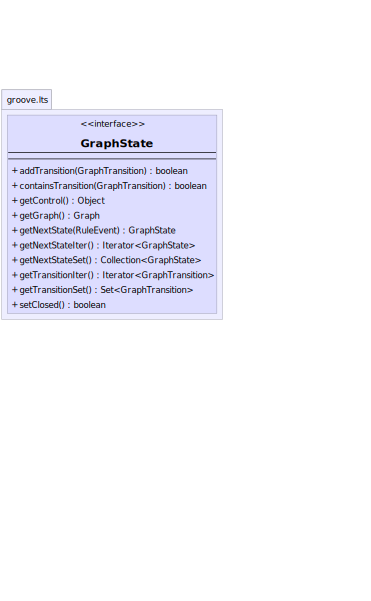
\includegraphics{fig/GraphState}
  \caption{Partial description of the interface {\tt lts.GraphState}.}
  \flabel{graphstate}
\end{figure}

\subsection{Storing a Labelled Transition System}

A labelled transition system is stored in an object of class {\tt lts.GTS}
(for Graph Transition System, i.e. transition system which states are
graphs), which implements {\tt lts.LTS}.

Let us first give an intuitive explanation of the way a LTS is stored.
Given an LTS $\mathcal S = (S, T, s_0)$, a {\em spanning tree} of $\mathcal
S$ is a tree whose set of nodes is $S$, has $s_0$ as a root, and whose
arrows are transitions in $T$ (see \fref{spanning tree} for an example of a
spanning tree). That is, a spanning tree contains all nodes of a LTS, but
not all transitions. However, if for any node we have sufficient
information allowing to reconstruct its outgoing transitions, then we can
easily reconstruct the whole LTS from its spanning tree. Storing a LTS as
one of its spanning trees allows to save space if we can store the missing
transitions in an efficient way. Now, a spanning tree can be completely
defined by its root and its set of nodes, if any node contains also its
unique (in the spanning tree) incoming arrow. This possibility is offered
by the interface {\tt lts.GraphNextState}.  We will see in the next section
how the possibility of efficient storage of an LTS by its spanning tree is
explored during the construction of an LTS.

\begin{figure}[ht]
  \centering
  
\includegraphics{fig/spanning-tree}
  \caption{A labelled transition system on the left and one of its spanning trees on the right.}
  \flabel{spanning tree}
\end{figure}

% \paragraph{Efficient Storage of Transitions in an LTS}
% As we mentioned previously, transitions of a GTS are stored as outgoing
% transitions by the states of the GTS. Therefore, it is not necessary to
% store the source state of a transition. The interface {\tt
%   lts.GraphOutTransition} describes transitions that do not know their
% source state. Its implementation {\tt lts.DefaultGraphOutTransition} thus
% defines a transition as a {\tt trans.RuleEvent} and a {\tt
%   lts.TargetState}. A {\tt trans.RuleEvent} is essentially a graph
% production and a host graph together with the image of the anchor of the
% left-hand side of the rule into the host graph. 

% \paragraph{Efficient Storage of States in an LTS}
% As described in \stref{storage of graphs}, several techniques are employed
% for efficient storage of graphs. Further optimisations can be done when
% graphs are the states of a LTS. A {\tt lts.GTS} stores its set of states as
% a set of objects of type {\tt lts.DerivedGraphState} (except for the start
% state).  As shown on \fref{states and transitions}, a {\tt
%   lts.DerivedGraphState} extends a {\tt graph.DeltaGraph}. Remind that a
% {\tt graph.DeltaGraph} stores a basis graph as well as an array of modified
% -- added and removed -- elements.  A {\tt lts.DerivedGraphState} contains
% information on its predecessor state in the spanning tree of the LTS and
% the corresponding incoming transition. The predecessor state is the basis
% graph. This transition contains the rule and the matching into the basis
% graph, thus removed elements can be deduced from it. Therefore, the delta
% array of a {\tt lts.DerivedGraphState} stores only the elements added to
% basis graph while performing the transition. These elements are also called
% {\em co-anchor image}: the image of the elements of the right-hand
% side of the rule that are new (w.r.t. the left-hand side).

\subsection{Constructing a Labelled Transition System}

The construction of a LTS is always done according to some exploration
strategy. In practise, the LTS corresponding to some graph grammar is often
infinite. Therefore, the strategy defines how to generate a portion of it
(e.g. depth-first, breadth-first). The strategy interface is given on
\fref{ExploreStrategy}.

\begin{figure}[ht]
  \centering
  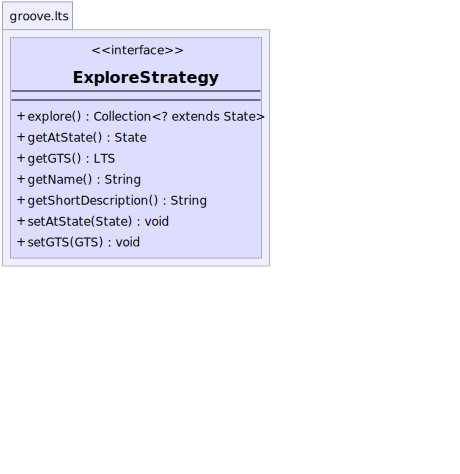
\includegraphics[scale=0.8]{fig/ExploreStrategy}
  \caption{The {\tt lts.ExploreStrategy} interface.}
  \flabel{ExploreStrategy}
\end{figure}

It allows to set the exploration at a given state ({\tt setAtState}) and to
make an exploration. For a list of the implemented strategies the reader is
invited to consult the {\em javadoc}.

The class {\tt lts.StateGenerator} that provides basic functionality for
generating new states in of a {\tt lts.GTS}, and is used as an interface by
the strategies. On \fref{StateGenerator} is depicted a partial view of the
functionality provided by this class.

\begin{figure}[ht]
  \centering
  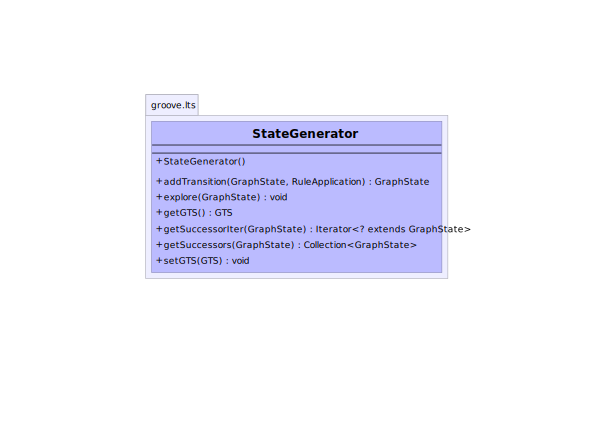
\includegraphics{fig/StateGenerator}
  \caption{Partial description of the class {\tt lts.StateGenerator}.}
  \flabel{StateGenerator}
\end{figure}

The method {\tt addTransition} adds a new transition to the associated GTS
(here a GTS) for the given source node and a {\tt trans.RuleApplication}.
The method {\tt explore} adds all (not already present) transitions to the
given state. Finally, the class gives to possibility to retrieve, or
iterate over, the successor states of a given state. 

% TODO
% We would like to describe here briefly different optimisation methods used
% while constructing the LTS.



% One can see that this class gives the possibility to compute the target
% state for some rule application, to add a transition to a LTS, or compute
% or iterate over all (already computed) successors of a given state. The
% protected method {\tt getConfluentTarget(RuleApplication)} is used for
% computing a successors state. It tries to derive the successor state
% walking around three sides of a confluent diamond instead of computing the
% state directly. When it is not possible, a {\tt lts.StateGenerator} uses a
% so called {\tt trans.Deriver} for performing the actual transformation.

% We give here only a brief description of derivers. More information can be
% find in the {\em javadoc}.

% On \fref{graph transitions} we show some hierarchies of classes used for
% representing a rule application.

% \begin{figure}[ht]
%   \centering
%   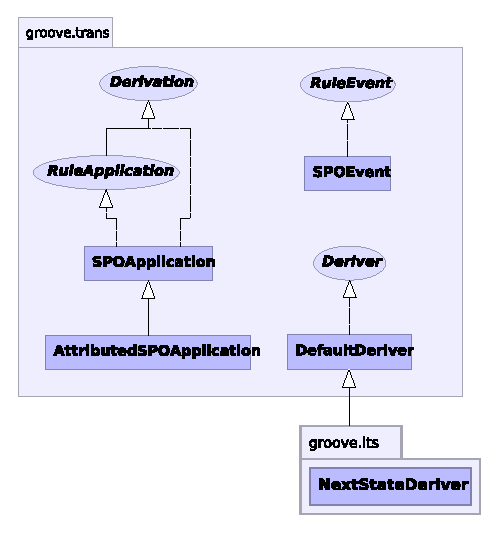
\includegraphics{fig/graph-transitions}
%   \caption{Hierarchy of classes for rule application.}
%   \flabel{graph transitions}
% \end{figure}

% Relative to the construction of the labelled transition system is the class
% {\tt lts.NextStateDeriver}. This is an implementation of a {\tt
%   trans.Deriver} that guarantees that newly generated graphs will be of
% type {\tt lts.DefaultNextState}. These is the run-time type of states of a
% {\tt lts.GTS}. Thus, a {\tt lts.StateGenerator} uses a {\tt
%   lts.NextStateDeriver} for computing graph derivations.




\addcontentsline{toc}{chapter}{Acknowledgments}
\chapter*{Acknowledgements}

UML diagrams in the present document are generated with the help of the
yDoc tool, by yWorks \url{http://www.yworks.com/en/products_ydoc.htm}.

\newpage
% Bibliography with BibTeX
% ========================
\bibliographystyle{abbrv}
\bibliography{references}

\end{document}
